\documentclass[a4paper,12pt,twoside]{article}
%\usepackage[american]{babel}
\usepackage{rotating}
\usepackage{epsfig}
\usepackage[centertags]{amsmath}
\usepackage{amscd}
\usepackage{array}
\usepackage{multirow}
\usepackage{supertabular}
\usepackage{colordvi}
\usepackage{dcolumn}
\usepackage{xspace}
\usepackage{lscape}

\begin{document}
\thispagestyle{empty}
\title{\bf Definition of geometries from external files in MaGe}
\author{Luciano Pandola}
\date{Version 0.0}
\date{\today}
\maketitle

\newcommand{\mage}{\textsc{MaGe} }

\section{Introduction}
The possibility to define a simple geometry by an external text file has 
been recently introduced in the \mage framework. The requirement for 
such a capability mainly comes from the need to roughly evaluate the 
detection efficiency in simple configurations. One instance is the probability 
that a $\gamma$-ray from a background source dissolved in liquid 
argon gives a full-energy deposition in a naked detector. While the 
precise evaluation of the efficiency requires a precise description of the 
whole experimental setup, that must be coded in \textsc{C++} and included 
in the directories \texttt{gerdageometry}, \texttt{mjgeometry} or 
\texttt{munichteststand}, a first order-of-magnitude estimate can be performed 
using the new feature, without editing or re-compiling the \mage code. 
This is particularly useful for non MC experts wishing to get a feeling of 
the efficiency of a given setup. \\
The results have been compared with those obtained using the \textsc{Teff} 
code, developed by V.~Tretyak. 
%
\section{Material definition} \label{material}
The \mage program already contains a list of commonly-used materials, that 
are coded in a local file, or read from a remote database. An arbitrary 
number of new materials can be defined using external files. The complete 
list of the materials defined in \mage can be obtained interactively 
using the command \\
\texttt{/MG/geometry/dumpG4materials} \\
given after the run initialization. 
A new material read from file is registered using the command \\
\texttt{/MG/geometry/addMaterial myfile.def} \\
where \texttt{myfile.def} is the external file containing the material 
definition. The command can be repeated several times, changing the file name, 
in order to define an arbitrary number of new materials. \\
An example of material definition file is the following: \\
\texttt{\\
SodiumIodide 3.67 2 \\
Sodium Na 11.0 22.989 0.153 \\
Iodine I 53.0 126.904 0.847 \\
\\}
In the first line, it must be specified:
\begin{itemize}
\item the name of the new material (string). It must be different from the 
names of the materials already defined in the \mage databases. If the 
user tries to re-define an existing material, the command is ignored, and 
a warning message is printed. 
\item material density, expressed in g/cm$^{3}$ (double).
\item number of elemental components (int).
\end{itemize}
The first line must be followed by the definition of the single elemental 
components. Their number must be equal to the one declared in the first line.
Each of the element lines is specified as follows:
\begin{itemize}
\item name of the element (string).
\item symbol of the element (string).
\item atomic number $Z$ (double).
\item average atomic mass $A$ (double)
\item mass fraction in the compound (double).
\end{itemize}
If an element with the same name is already defined in the \mage internal 
database, the re-definition from the file is ignored, and only the mass 
fraction is taken into account. A warning message is printed. The user 
must take care that the sum of the mass fractions is actually 1.0.
%
\section{Geometry definition} 
To switch on the geometry definition from an external file, the messenger 
command \\
\texttt{/MG/geometry/detector GeometryFile} \\
has to be given. The name of the file containing the geometry to be read 
is set using the command \\
\texttt{/MG/geometry/geometryFileName mygeometry.def} \\
If the command \texttt{/MG/geometry/geometryFileName} is issued more than 
once, the file name is overwritten, and the last one is taken into account. 
If the general geometry has not been set with the command 
\texttt{/MG/geometry/detector GeometryFile}, the file name is anyway accepted 
but it is not used. If the file name is not given explicitly, the default 
\texttt{geometry.def} is looked for in the current directory. \\
It is possible to define an arbitrary 
number of boxes, cylinders and spheres. Volumes can be daughters of the 
world or of an other volume. In the latter case, it is possible to define 
``holes'' in a given volume. \\
An example of geometry definition file is the following: \\
\texttt{\\
1 Crystal 2 1 0 SodiumIodide   \\
0. 0. 2.55 \\
2.55 5.10 0. \\
0. 0. 0. \\
2 Hole    2 0 1 Air\\             
0. 0. 0.65 \\
1.43 3.80 0.\\
0. 0. 0. \\
\\}
Each volume is defined in four lines. \\
(1) The entries for the first line are:
\begin{itemize}
\item ordering number (int).
\item volume name (string). This is the name of the physical volume defined 
in the geometry. It can be used, for instance, for the uniform sampling 
routine. The names of the volumes should be different, though there is no 
specific control in the program. 
\item shape of the volume (int). The code is 1 for boxes, 2 for cylinders and 
3 for spheres. If the code is different from the values listed above, the volume  
is ignored.
\item sensitive detector flag (int). If the flag is 1, the volume is 
registered as a sensitive detector for the subsequent analysis. 
\item mother flag (int). If the flag is set to 0, the volume is placed inside the 
world volume. If the flag is a non-zero integer $n$, the volume is considered 
to be a daughter of the volume $n$. The mother volume must be defined 
\emph{before} the daughter one (namely, the ordering number of the Daugherty 
must be larger than $n$). It is possible to nest daughter volumes one inside 
the other.
\item material name. The material has to be included in the \mage database 
or defined using an external file, as described in Sect.~\ref{material}.
\end{itemize}
(2) The second line contains the three coordinates of the volume center, given in cm (double). 
Coordinates are always expressed with respect to the mother volume reference system. \\
(3) The third line contains the three physical dimensions of the volume (double), given in cm. 
For boxes, the numbers are the sizes along the $x$, $y$ and $z$ axes, respectively. 
For cylinders, the first parameter is the radius, and the second the height (the 
third parameter is unused).  
For spheres, the first parameter is the radius, the other two are unused. \\
(4) The fourth line contains the three Euler angles (degrees) defining the volume rotation. 
The angles are always referred to the mother volume reference system. \\
The volumes defined in the external file are placed in a world volume made of air. The 
world volume is a cube of 5~m size. Therefore, the dimensions of the volumes in 
the file cannot exceed 5~m.\\
The geometry file presented above represents: a cylindrical sodium iodide detector (radius 
2.55~cm, height 5.10~cm) with a cylindrical hole (radius 1.43~cm, height 3.8~cm) displaced 
of 0.65~cm along the $z$-coordinate of the detector. The coordinates of the center of the 
detector are (0,0,2.55~cm) with respect to the world reference frame. The sketch of the 
geometry is displayed in Fig.~\ref{testgeometry}. \\
%%
\nopagebreak
\begin{figure}[tb]
\begin{center}
\mbox{\epsfig{file=geom.eps,height=10cm}}
\caption{Sketch of the setup geometry defined in \textsc{MaGe} with the external 
data files used as example in the text.}\label{testgeometry}
\end{center}
\end{figure}
%
\section{Analysis}
The analysis of the Monte Carlo data can be performed using an output scheme 
of \textsc{MaGe}, and depends on the information that the user wants to extract. A 
specific output scheme is available in \mage for the evaluation of the efficiency of the 
detectors that are registered as sensitive. The general-purpose output scheme for 
the efficiency is instantiated with the command: \\
\texttt{/MG/eventaction/rootschema DetectorEfficiency} \\
It gives in output a single ASCII file, whose name is set with the command: \\
\texttt{/MG/eventaction/rootfilename myoutput.dat}\\
If the output file name is not set explicitly, the default \texttt{output\_eff.dat} 
is created. \\
The output ASCII file is a 4-column table. The columns contain:
\begin{enumerate}
\item the energy of the primary particles;
\item the total number of generated primary tracks;
\item the number of events having an energy deposition in the sensitive detector;
\item the number of events having full energy deposition in the sensitive detector.
\end{enumerate}
An event is considered as a full-energy deposition if the energy deposited in the sensitive 
detector is equal to the primary energy, within 1~keV tolerance. 
%
\section{Full application} \label{themacro}
Here is presented, as an example, a \textsc{MaGe} macro to evaluate the efficiency of the 
sodium iodide detector of Fig.~\ref{testgeometry} for point-like $\gamma$-ray sources of different 
energies placed in the hole. \\
\texttt{\\
/MG/manager/mglog trace \\
\# \\
/MG/geometry/detector GeometryFile\\
/MG/geometry/database false\\
/MG/geometry/addMaterial sodiumiodide.def\\
/MG/geometry/geometryFileName geometry.def\\
\# \\
/MG/eventaction/rootschema DetectorEfficiency\\
/MG/eventaction/rootfilename output.dat\\
\# \\
/MG/processes/lowenergy true\\
/MG/processes/realm DarkMatter\\
\# \\
/run/initialize\\
\# \\
/MG/generator/select G4gun \\
/gun/particle gamma\\
/gun/position 0. 0. 1.4 cm\\
/MG/generator/g4gun/cone\_on true\\
/MG/generator/g4gun/coneDirection 0 0 -1\\
/MG/generator/g4gun/thetaDelta 180 deg\\
\# \\
/gun/energy 100 keV\\
/run/beamOn 10000\\
/gun/energy 200 keV\\
/run/beamOn 10000\\
/gun/energy 300 keV\\
/run/beamOn 10000\\
$\ldots$\\
\\}
The first command, \texttt{/MG/manager/mglog trace} is used to set the verbosity level of \mage 
(namely, the quantity of information that is given in the interactive output). \\
The block \\ 
\texttt{
/MG/geometry/detector GeometryFile\\
/MG/geometry/database false\\
/MG/geometry/addMaterial sodiumiodide.def\\
/MG/geometry/geometryFileName geometry.def\\
}
is used to define the geometry. The \mage material database is read from the local file 
(rather than remotely from the Majorana database) and a new material is read from the file 
\texttt{sodiumiodide.def}. The geometry is read from the file \texttt{geometry.def}. \\
The block \\
\texttt{
/MG/eventaction/rootschema DetectorEfficiency\\
/MG/eventaction/rootfilename output.dat\\
}
sets the output scheme and the name of the output file. The physics of the simulation is set in 
the block\\
\texttt{
/MG/processes/lowenergy true\\
/MG/processes/realm DarkMatter\\}
With the first line the user requires that the electromagnetic processes are treated according to 
the specific low-energy models of \textsc{Geant4}. The low-energy models, that include fluorescence 
and other atomic effects, are more precise than the standard \textsc{Geant4} electromagnetic processes 
but typically slower. The second line sets the cut for the generation of $\delta$-ray and of 
bremsstrahlung photons. With the \texttt{DarkMatter} option, the cuts are small, and the tracking is 
extremely accurate (and slow). More relaxed cuts can be set with the \texttt{DoubleBeta} and 
\texttt{CosmicRays} options. The command 
\texttt{/run/initialize} is then issued to initialize the \mage run.
After that, the block\\
\texttt{ 
/MG/generator/select G4gun \\
/gun/particle gamma\\
/gun/position 0. 0. 1.4 cm\\
/MG/generator/g4gun/cone\_on true\\
/MG/generator/g4gun/coneDirection 0 0 -1\\
/MG/generator/g4gun/thetaDelta 180 deg\\}
is used to define the primary particles. The generator is set to be \texttt{G4gun}, which is the 
default \texttt{G4ParticleGun} generator provided by \textsc{Geant4}. The second and third lines 
define the particle type ($\gamma$-ray) and position, respectively. The coordinates of the source 
are defined in the world reference system. It is possible to use the existing \mage capabilities 
to generate primary particles uniformly from a given volume\footnote{
For instance, the commands\\
\texttt{
/MG/generator/confine volume \\
/MG/generator/volume Crystal \\}
would generate primary particles uniformly distributed in the volume named Crystal.}. The sub-set \\
\texttt{
/MG/generator/g4gun/cone\_on true\\
/MG/generator/g4gun/coneDirection 0 0 -1\\
/MG/generator/g4gun/thetaDelta 180 deg\\
}
defines the angular distribution of the primary $\gamma$-rays. The $\gamma$-rays are generated 
isotropically in a cone, whose axis is the $z$ axis and the opening angle is 180 degrees. This is 
a way to generate an isotropic flux from the source. \\
\texttt{
/gun/energy 100 keV\\
/run/beamOn 10000\\
/gun/energy 200 keV\\
/run/beamOn 10000\\}
Eventually, the user sets the particle energy to 100~keV and shoots 10~000 events, then to 200~keV 
and shoots 10~000 events, and so on. The procedure can be repeated for an arbitrary number of times, 
changing the primary energy (and possibly the particle type and position). 
%
\section{Comparison}
The results obtained by \mage for the simpled geometry sketched in Fig~\ref{testgeometry} running 
the macro discussed in Sect.~\ref{themacro} have been compared with those obtained using the 
code \textsc{Teff} by Vladimir Tretyak for the same setup. Fig.~\ref{teff} 
(courtesy of V.~Tretyak) shows 
the profile of the full efficiency (= any energy deposition in the detector) vs. energy obtained 
using \mage and \textsc{Teff}. The results are in good agreement.
%%
\nopagebreak
\begin{figure}[tb]
\begin{center}
\mbox{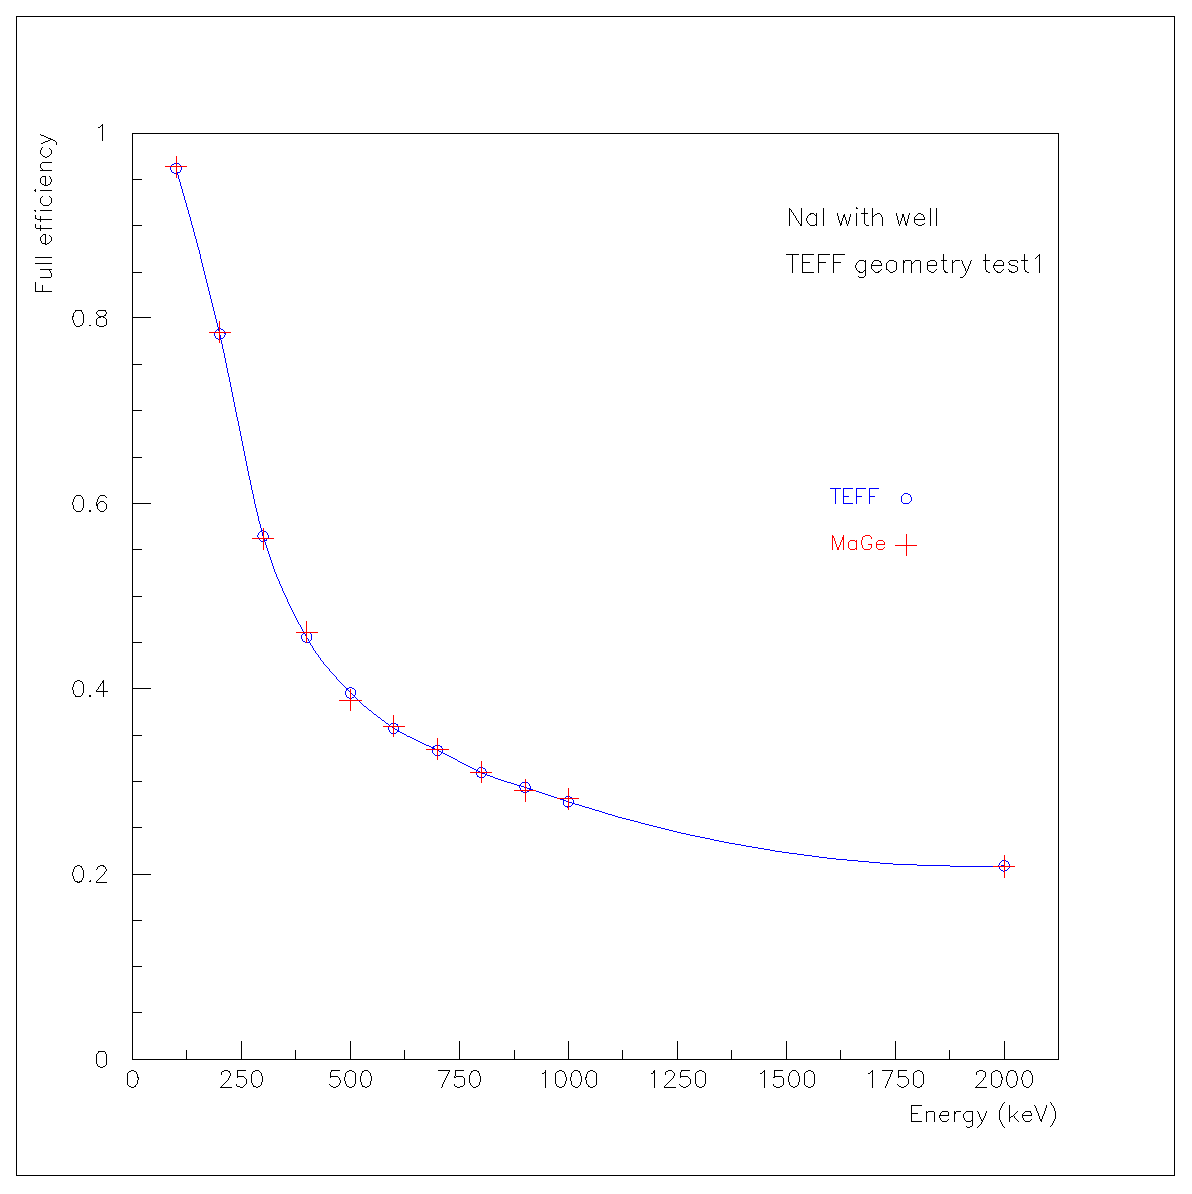
\epsfig{file=mage2.eps,height=15cm}}
\caption{Total efficiency for a point-like $\gamma$-ray source in the setup shown in 
Fig.~\ref{testgeometry} using \textsc{MaGe} and \textsc{Teff} (courtesy of Vladimir 
Tretyak). The efficiency represents 
the probability that the $\gamma$-ray interacts in the NaI sensitive volume, with any 
energy release (full peak + Compton continuum).}\label{teff}
\end{center}
\end{figure}
%

\end{document}
